\documentclass[10pt]{article}
\usepackage[a4paper,margin=2.0cm]{geometry}
\usepackage[T1]{fontenc}
\usepackage{lmodern}
\usepackage{microtype}
\usepackage{amsmath}
\usepackage{booktabs}
\usepackage{graphicx}
\usepackage{caption}
\usepackage{float}
\usepackage[hidelinks]{hyperref}
\setlength{\parskip}{0.45em}
\setlength{\parindent}{0pt}
\captionsetup{font=small,labelfont=bf}

\title{\vspace{-1.6em}Equal quality: the same image in less time, and the effect of emitter resolution}
\author{}
\date{\vspace{-2.4em}}

\begin{document}
\maketitle
\vspace{-1.0em}

\textbf{Summary.} Comparing techniques by RMSE at equal frame time understates what a cheaper sampler provides, because image error stops improving once light-sampling noise is no longer its main part. We therefore also ask the converse question: how long does each technique need to reach the quality that the 2D CDF delivers in a 33.3\,ms frame? Over full videos of the five scenes, BudgetLeafAlias is 1.19 to 2.23 times faster and CodecLeafAlias 1.23 to 2.31 times faster. The advantage grows with the resolution of the emitter: on an LED wall showing an 8K photograph, a light sample costs the 2D CDF three times more than at Full HD and our techniques 1.5 times more, so that both reach the 2D CDF's quality \textbf{3 times faster}, or give \textbf{21\% lower RMSE in the same 33.3\,ms}.

\section*{1\quad Why equal quality}

With $n$ light samples per shading point, the error of a frame behaves as $\mathrm{MSE} = a + b/n$, where $b/n$ is the noise of light sampling and $a$ is everything that light samples do not reduce at the scene's samples per pixel. The RMSE therefore flattens quickly: in Rover it is 0.090 with 1 light sample, 0.045 with 32 and 0.042 with 64, for every technique. Near that floor, a technique that affords 1.7 times the samples of another in the same time gains only about 5\% in RMSE. The cost reading does not have this compression. At equal samples all importance-sampling techniques are within a few percent of each other (see the equal-samples study), so they need about the same number of samples for a given quality, and the faster sampler delivers it in less time. That time can be returned to the frame rate, to more bounces, or to a denoiser.

\section*{2\quad The five scenes}

For each scene we render frames spanning its whole video (60--120 frames) with direct illumination, where the light sampler controls most of the noise, and compare each frame with a converged reference. The 2D CDF uses the number of light samples that fits a 33.3\,ms frame. Every other technique is rendered with several numbers of light samples, and we find the frame time at which its video RMSE equals that of the 2D CDF. The speedup is the frame time of the 2D CDF divided by that time: the same image quality, delivered faster. Frame times are medians over the timing passes of each scene.

\begin{table}[H]
\centering\small
\caption{Speedup over the 2D CDF at equal quality on the five scenes (full videos, direct illumination): the frame time of the 2D CDF divided by the frame time each technique needs to reach the same video RMSE. Above 1 is faster than the 2D CDF. --: the technique does not reach the 2D CDF's quality at the measured points.}
\label{tab:scenes}
\begin{tabular}{lccccc}
\toprule
Technique & Rover & Cinema & Fireplace Room & Phone & Convergence \\
\midrule
2D CDF & 1.00 & 1.00 & 1.00 & 1.00 & 1.00 \\
2D CDF/8 & 1.17 & 1.89 & 1.29 & 1.17 & 1.17 \\
Mipmap & 0.85 & 1.45 & 1.10 & -- & 1.06 \\
Alias per pixel & 1.17 & 1.91 & 0.91 & 1.26 & 0.93 \\
\textbf{BudgetLeafAlias} & 1.31 & 2.23 & 1.19 & 1.47 & 1.27 \\
\textbf{CodecLeafAlias} & 1.38 & 2.31 & 1.54 & 1.23 & 1.37 \\
\bottomrule
\end{tabular}
\end{table}


\textbf{Our two techniques reach the quality of the 2D CDF faster on all five scenes}: BudgetLeafAlias by 1.19 to 2.23 times and CodecLeafAlias by 1.23 to 2.31 times (Table~\ref{tab:scenes}). The quality that the 2D CDF delivers at 30 frames per second is delivered at 36--67 frames per second by BudgetLeafAlias and at 37--69 by CodecLeafAlias. One of the two is the fastest technique on every scene. The other techniques are not consistent: the mipmap warp is slower than the 2D CDF on Rover, and the per-pixel alias table, which is fast on Full HD emitters, is slower than the 2D CDF on the two scenes with 4K emitters, where its table has grown to 166\,MB.

\section*{3\quad A harder case: an 8K LED wall}

The last observation suggests that the resolution of the emitter decides the size of the advantage. To isolate it, we show the same photograph at three resolutions on the LED wall of the Rover scene: 1820$\times$1024, 3640$\times$2048 and 7280$\times$4096, obtained by area averaging from a real 8K HDR panorama (16:9 crop of the horizon band). We use two photographs: a road under broad daylight, where the light is spread over the whole image, and a morning landscape with the sun in frame, where a few texels hold about half of the emitted power.

\emph{Setup.} One frame, direct illumination, 1920$\times$1080 render. For each technique we measure frame time and RMSE (8 renders against a converged reference) at 16 light-sample counts from 1 to 64 per shading point, the engine's limit. Frame times are interpolated between measured counts, and the RMSE curve of each technique is smoothed with a quadratic fit in logarithmic axes (residual about 2\%). BudgetLeafAlias uses 4000 leaves at all resolutions.

\begin{table}[H]
\centering\small
\setlength{\tabcolsep}{4pt}
\caption{LED wall showing the same photograph at three resolutions (Rover scene, one frame, direct illumination). \emph{samples}: light samples per shading point that fit in a 33.3\,ms frame (+: the engine's limit of 64 is reached before 33.3\,ms). \emph{faster}: how many times shorter the frame is than the 2D CDF's 33.3\,ms when the technique reaches the same RMSE. \emph{RMSE}: error at 33.3\,ms relative to the 2D CDF (below 1 is better). $^\dagger$Not reported: see the text.}
\label{tab:wall}
\begin{tabular}{l ccc ccc ccc}
\toprule
 & \multicolumn{3}{c}{1820$\times$1024} & \multicolumn{3}{c}{3640$\times$2048} & \multicolumn{3}{c}{7280$\times$4096} \\
\cmidrule(lr){2-4}\cmidrule(lr){5-7}\cmidrule(lr){8-10}
Technique & samples & faster & RMSE & samples & faster & RMSE & samples & faster & RMSE \\
\midrule
\multicolumn{10}{l}{\textit{Road, broad light}} \\
2D CDF & 34 & 1 & 1 & 25 & 1 & 1 & 10 & 1 & 1 \\
2D CDF/8 & 45 & 1.33 & 0.939 & 38 & 1.58 & 0.916 & 32 & 2.67 & 0.814 \\
Mipmap & 33 & 0.98 & 1.004 & 31 & 1.06 & 0.957 & 28 & 2.44 & 0.826 \\
Alias per pixel & 53 & 1.52 & 0.917 & 22 & 0.93 & 1.014 & 16 & 1.49 & 0.915 \\
\textbf{BudgetLeafAlias} & 60 & 1.78 & 0.883 & 58 & 2.15 & 0.852 & 40 & 3.08 & 0.792 \\
\textbf{CodecLeafAlias} & 59 & 1.67 & 0.901 & 55 & 2.04 & 0.871 & 40 & 3.06 & 0.791 \\
\midrule
\multicolumn{10}{l}{\textit{Morning, sun in frame}} \\
2D CDF & 46 & 1 & 1 & 35 & 1 & 1 & 22 & 1 & 1 \\
2D CDF/8 & 57 & 1.22 & 0.957 & 51 & 1.41 & 0.927 & 46 & 1.95 & 0.864 \\
Mipmap & 39 & 0.88 & 1.031 & 38 & 1.11 & 0.978 & 36 & 1.71 & 0.899 \\
Alias per pixel & 64+ & 1.37 & 0.927 & 33 & 0.95 & 1.011 & 27 & 1.23 & 0.957 \\
\textbf{BudgetLeafAlias}$^\dagger$ & -- & -- & -- & -- & -- & -- & -- & -- & -- \\
\textbf{CodecLeafAlias} & 64+ & 1.51 & 0.939 & 64+ & 1.76 & 0.893 & 63 & 2.38 & 0.819 \\
\bottomrule
\end{tabular}
\end{table}


\begin{figure}[H]
\centering
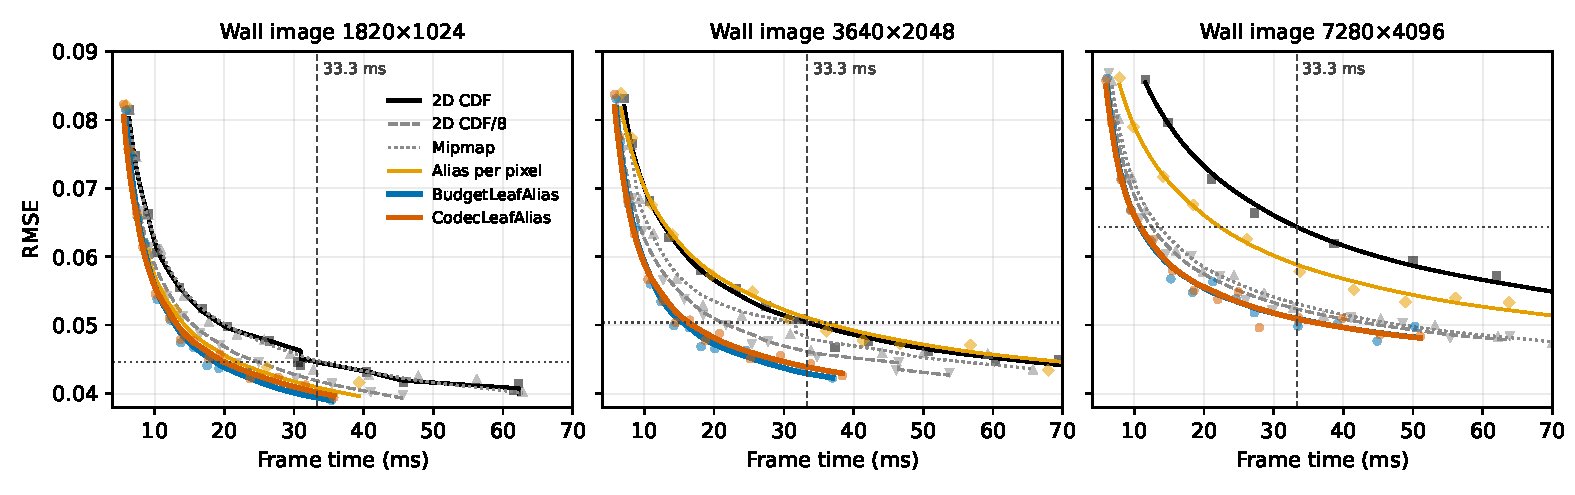
\includegraphics[width=\textwidth]{fig_wall.pdf}
\caption{Road photograph on the LED wall: RMSE against frame time at the three resolutions (markers: measurements; curves: fits). The vertical line is the 33.3\,ms budget and the horizontal line the RMSE of the 2D CDF at that budget. As the image grows, the curve of the 2D CDF moves to the right and ours stay almost in place.}
\label{fig:wall}
\end{figure}

\textbf{The cost of a light sample grows with resolution for the 2D CDF, and much less for our techniques.} On the road photograph, each additional light sample per shading point adds 0.95, 1.17 and 2.93\,ms to the frame of the 2D CDF at the three resolutions, and 0.47, 0.50 and 0.73\,ms to that of BudgetLeafAlias (0.49, 0.53, 0.75 for CodecLeafAlias). The 2D CDF searches a table as large as the image, with one dependent memory read per search step, and at 8K that table is sixteen times larger than at Full HD; ours read a tree and a table of about 75\,KB at any resolution, and the image only once the texel has been chosen. In a 33.3\,ms frame the 2D CDF therefore fits 34, 25 and 10 light samples, while BudgetLeafAlias fits 60, 58 and 40 (Table~\ref{tab:wall}).

\textbf{The speed-up at equal quality grows from 1.8 times at Full HD to 3.1 times at 8K.} BudgetLeafAlias reaches the quality of the 2D CDF's 33.3\,ms frame 1.78, 2.15 and 3.08 times faster at the three resolutions, and CodecLeafAlias 1.67, 2.04 and 3.06 times faster: at 8K, about 11\,ms instead of 33.3. Read at equal time, the RMSE of BudgetLeafAlias is 12\%, 15\% and 21\% lower than the 2D CDF's, the largest equal-time difference in all our tests; it is this large because at 8K the 2D CDF is left with so few samples that it is still far from the noise floor. Our two techniques are the fastest at every resolution.

The per-pixel alias table follows the 2D CDF: fast at Full HD (1.52), it becomes slower than the 2D CDF at 4K (0.93) and recovers only part of the difference at 8K (1.49), since its table also grows with the image. The two baselines that keep small or hierarchical structures, the 2D CDF at one eighth of the resolution and the mipmap warp, scale better and reach 2.67 and 2.44 times at 8K; they remain behind our techniques at every resolution, and the reduced 2D CDF obtains its speed by giving up resolution, which costs it up to 2.6\% in RMSE at equal samples on the five scenes (see the equal-samples study).

\emph{Sun in frame.} On the morning photograph the pattern is the same and milder, since most samples fall on the few texels of the sun, which stay in cache: the cost of a sample goes from 0.63 to 1.35\,ms for the 2D CDF and from 0.38 to 0.46\,ms for CodecLeafAlias, which is again the fastest technique at every resolution: it reaches the 2D CDF's quality 1.51, 1.76 and 2.38 times faster and has 6\%, 11\% and 18\% lower RMSE at equal time. BudgetLeafAlias is not reported on this image: its current implementation stores the mean luminance of a leaf as a 16-bit float, which saturates at 65504, and the sun texels of this photograph reach 148000. This is a storage limit of the implementation and not of the partition, and it does not affect the five scenes, whose videos stay far below that value.

\emph{Scope.} The wall test uses a single frame, direct illumination and one timing pass per technique. With full global illumination the noise that light samples do not reduce is larger, and the factors at equal quality are expected to be smaller, as they are at equal time. The trend with resolution is consistent across both photographs and all techniques that keep a full-resolution table.

\end{document}
